% !TEX root = main.tex
\chapter{Rocket Tests}\label{cha:experimental}

	MEOWTH II was tested at Peter Madsen's space laboratory in Copenhagen, on the 3rd to the 4th of May 2016 by Team Rocket of Navitas. The whole ordeal has spawned several articles, which the interested reader can find in appendix \ref{App:A}. A  complete logbook along with a firing procedure can be found in appendix \ref{App:B}.

	The test setup can be seen in figure \ref{fig:rocketpic}, and the first burn can be seen on the front page. The test stand consists of a metal fixture that holds the rocket in a horizontal position, with the hydrogen--peroxide tank standing vertically. The metal fixture keeps the rocket from moving under tests. Sandbags are placed on top in order to stop fast--moving shrapnel, in case of a complete engine destruction. Further safety instructions can also be found in appendix \ref{App:B}.

	The purpose of the experiments was to measure the variations in pressure throughout the rocket. The following will be an analysis of the data collected, along with a brief description of the sensors involved. A group consisting of three students also took video footage of the tests in order to analyze the rocket's shock diamonds, this will not be treated here, however.

	\section{Equipment}

	Eight pressure sensors were mounted on the rocket, ranging over three measurement frequencies: $\SI{250}{\Hz}$, $\SI{2000}{\Hz}$ and $\SI{20000}{\Hz}$. All were measured at $\SI{20000}{\Hz}$, which means the slower sensors are oversampled. One of each sensor was placed in both the rocket's mixing chamber and decomposition chamber. The two remaining sensors, a slow and a fast, were mounted by the hydrogen--peroxide tank. The measurement equipment was connected to a DAta Acquisition (DAQ) system from National Instruments, which in turn was connected to the data--logging software LabVIEW on a nearby slave unit. The slave unit was remotely controlled by a computer inside the safety--submarine, which allowed ignition and data--logging nearby the test site without being in danger.

	Two manometers were placed before and after the pressurization valve, in order to manually check the tank's pressure before ignition.

	A more thorough discussion of project improvements can be found in chapter \ref{cha:perspective}. A more thorough discussion of individual sensors and specific sensor result can be found in my brother--groups report here: \url{https://github.com/carlegroen/bachelors_degree/tree/master/cousinprojects/}.

	\section{Experimental Procedure}

	\begin{figure}
		\centering
		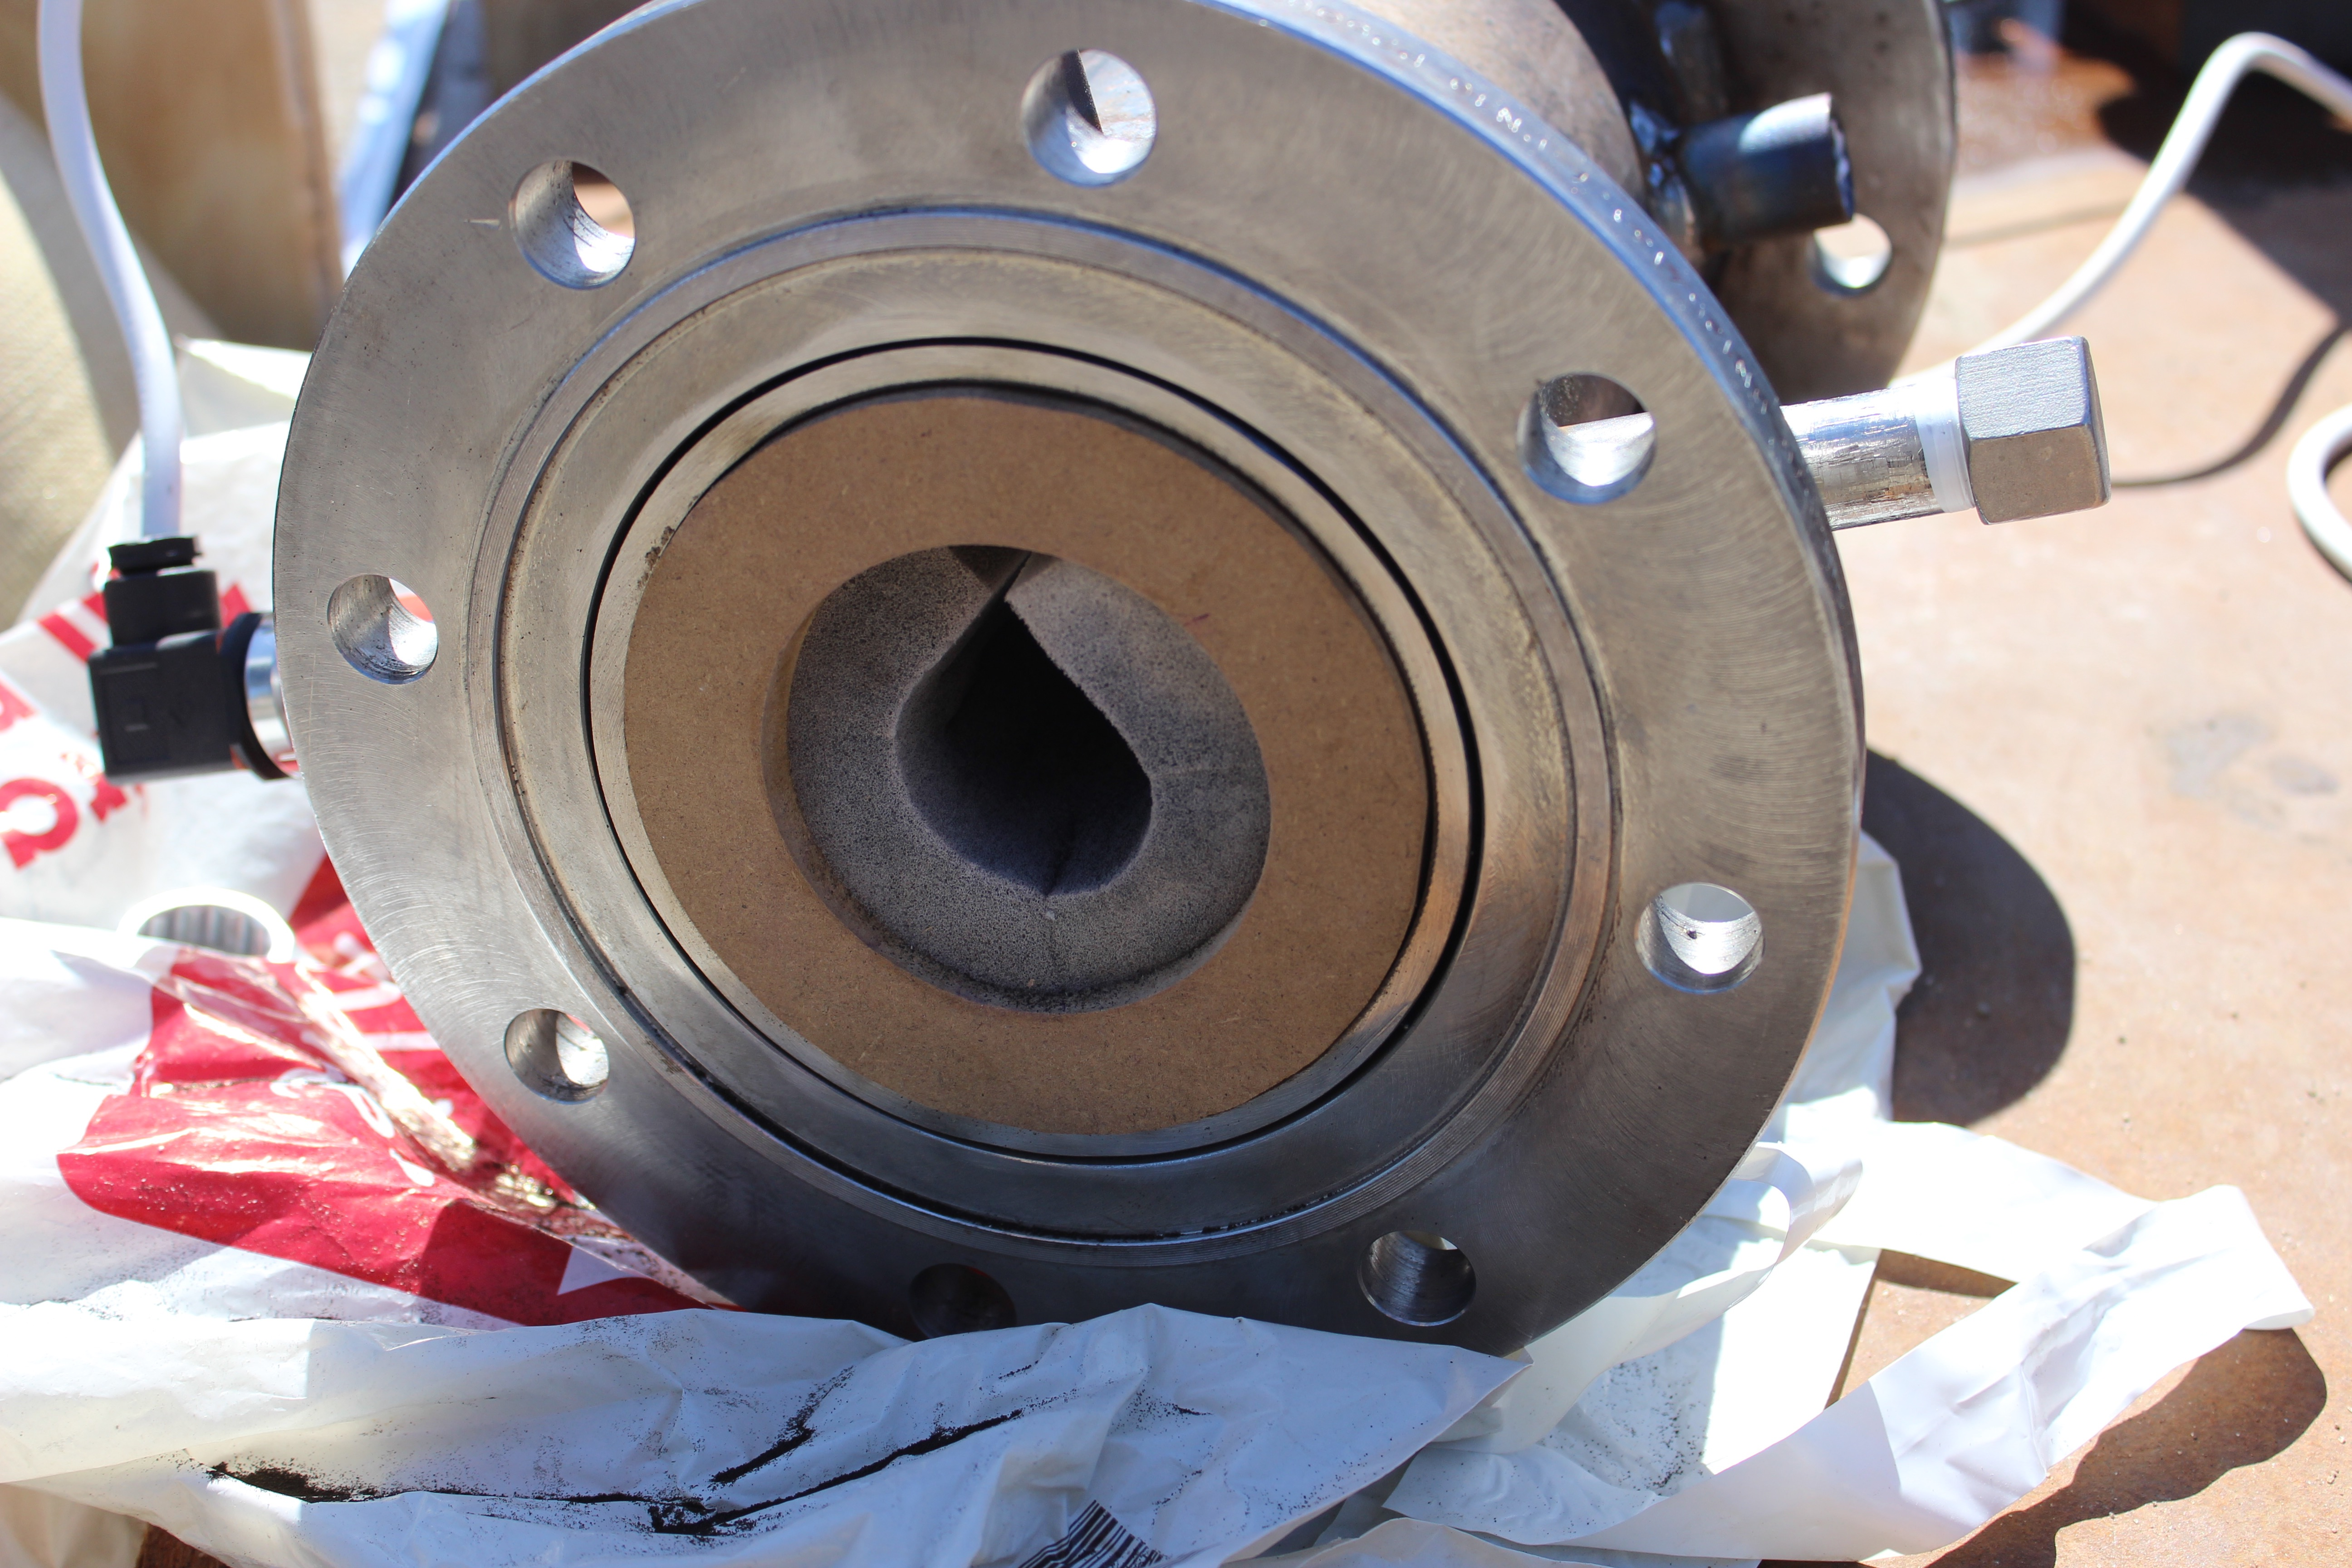
\includegraphics[width=\textwidth]{decompchamber}
		\caption{Foam permeated with \chem{KMnO_4} dust inserted into the decomposition chamber, inside a tube of MDF, in order to avoid accumulation of liquid \chem{H_2 O_2}}
		\label{fig:kmno4foam2}
	\end{figure}

	MEOWTH II was built specifically with the intent of being fast to rearm. The large flanges allows quick unbolting, and the hydrogen--peroxide tank has a quick-fill valve. The only swappable objects which changes the combustion rate is the decomposition nozzle and the fuel--grain. The tank's pressurization changed throughout the experiments, which greatly influences the flow--rate of hydrogen--peroxide. An analysis of the tank's pressure's influence on flow--rate has not been executed, however, that could be a subject for a future project. The wagon--wheel fuel grain design (see figure \ref{fig:wagonwheel}) was kept throughout the experiments, which makes the decomposition nozzle the only variable in the experiments.

	Apart from changing larger parts of the experimental setup, reloading proceduce requires swapping the rocket's interior. In figure \ref{fig:kmno4foam2}, the decomposition chamber is visible with its inner MDF--shell casing, filled with \chem{KMnO_4}--permeated foam. The inner casing prevents liquid puddles from not building up and causing trouble, in the form of instant vapourization into large quantities of gas.

	\begin{figure}
		\centering
		\includegraphics[width=\textwidth]{wagonwheelburnt}
		\caption{Wagon-wheel shaped grain as seen in figure \ref{fig:wagonwheel} after a test. Notice the wagon-wheel pattern has been burnt through, and instead a "flower"--pattern is present. Experimentally this can be seen as a small drop in pressure as seen in the results.}
		\label{fig:burntgrain}
	\end{figure}

	Swapping the wagon-wheel grain with an identical copy after every test is essential to receive consistent results, as it is worn greatly during combustion. As seen in figure \ref{fig:burntgrain}, the grain's inner walls are burnt through about two--thirds through every test. This greatly influences the grain's regression--rate, making new-- and old--grain experiments vastly different.

	Preliminary tests were done with water, as to check the newly made decomposition nozzle. Testing with water also showed leaks, making it easier to tighten and seal the piping before loading the toxic high--concentration hydrogen--peroxide. After preliminary tests, four tests were concluded and will be discussed below.

	\section{Results}
	
	All tests used $\SI{1.3}{\liter}$ of hydrogen--peroxide, making the injection rate easy to calculate assuming linear flow.	In figure \ref{fig:burnresults} the resulting pressure over time graphs are seen. As seen in the figure, higher tank pressure appears to influence the spike's height. It is questionable whether or not the spike in test three and four are representative, as data on the top appears "flattened", as if the pressure went further than the set measurement range for a brief amount of time. After the spike, the graphs flatten out and slowly decrease until they all drop slightly in pressure. This drop is most likely due to the grain's design. The wagon-wheel design seen in figure \ref{fig:wagonwheel} has a large surface area for combustion. After burning for some time the grain's wall regress far enough to create a larger cavity, but drop in overall surface area as the walls collapses to a flower--pattern as seen in figure \ref{fig:burntgrain}. As the walls are burnt through, the surface area decreases and in turn, so does the regression--rate and combustion rate. This reduces the chamber pressure by approximately $20\%$. 
	
	As the rocket is ignited noise starts to arise. This gives a clear indicator of when rocket ignition happens, but at the cost of accuracy. The noise was an unwanted feature, which stems from an accidental ground-loop in the test--setup. The rocket burns are all zeroed around the noise which shows when ignition starts after opening the ball--valve. 
	
	The first test shows a significantly slower ignition than the three others, which is most likely due to the flanges not being tightened correctly, leaking gas out the sides. Test 2 and 3 have almost identical ignition timing, although their tank--pressures differ by $\SI{7}{\bar}$. Their injectors are identical, which makes the change in spike size and timing dependent on the mass flow. It also appears that test 2 and 3 have a duration difference of almost 1 second, which is given only by the change in pressure. 
	The final test have identical tank--pressure to test 3, but with an injector with higher flow--rate. The size of the spikes are seemingly identical, however, upon further inspection it appears that the peaks are flattened due to a too low sample--range. Thus, the peak heights are not exactly representative. Interestingly, the time before ignition happens is shorter with the higher flow--rate injector. It is also quite visible that test 4 concludes much faster than the rest, after only approximately 4 seconds from initial injection, compared to the usual 6 to 8 seconds.

	\begin{figure}
		\centering
		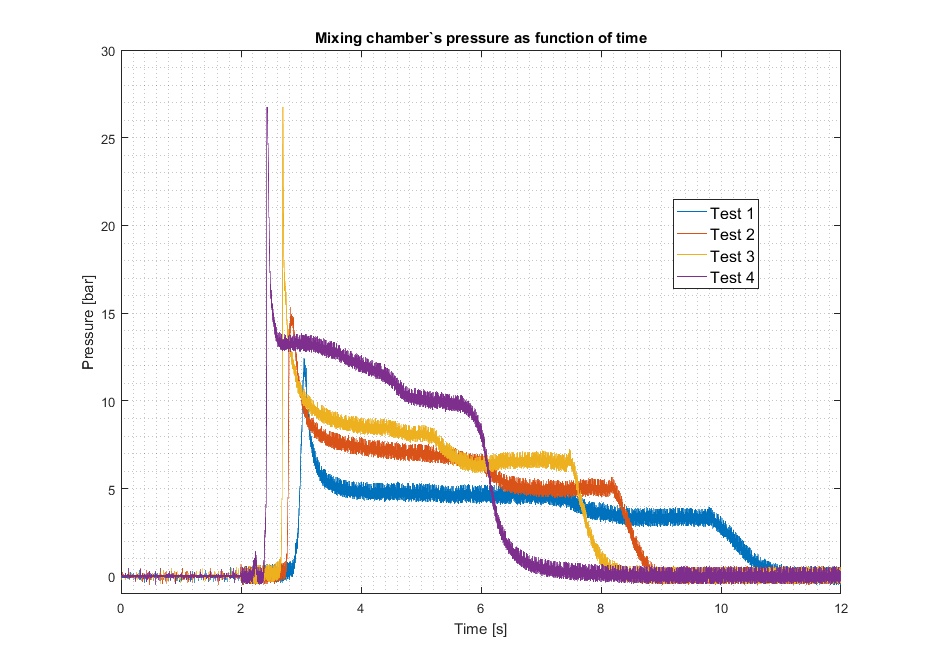
\includegraphics[width=\textwidth]{burnresults}
		\caption{Results from the four tests. Test one through four was done with pressures of $\SI{24}{\bar}, \SI{24}{\bar}, \SI{31}{\bar}$ and $\SI{31}{\bar}$ respectively. The last test was done with a larger injector.}
	\label{fig:burnresults}
	\end{figure}


% Testing of the rocket engine ensued at "Raketmadsens Rumlaboratorium" in Copenhagen on the 3rd to the 4th of may 2016. The tests were carried out by me in company by my advisor Gorm Bruun Andresen, and seven other students from Navitas.
%

%

%
% \section{Results}
%
% A total of ten measurements were collected at every test. The most essential is the Piezoelectric pressure sensors located at the front. The simulation calculates the pressure after the combustion chamber, and at the nozzle's exit.
%
% \begin{figure}
% 	\centering
% 	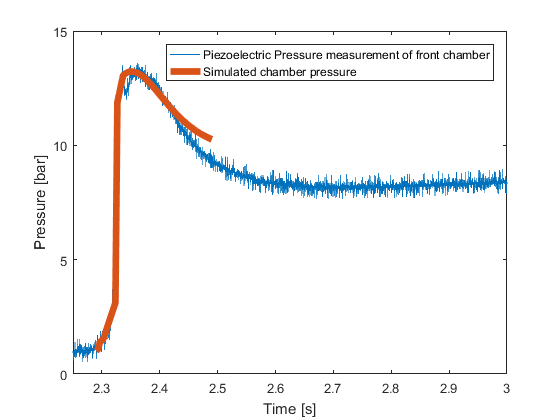
\includegraphics[width=\textwidth]{peakBurn2wsim}
% 	\caption{The second burn's front chamber peak, as found by the Piezoelectric pressure sensor. Plotted on top is the simulation created in this bachelor's thesis.}
% 	\label{fig:peakBurn2wsim}
% \end{figure}
%
% The experimental and simulation results are seen in figure \ref{fig:peakBurn2wsim}, where the blue line is the experimental results, and the red is the simulated pressure. The simulation assumes no combustion until a temperature of $\SI{220}{\celsius}$, at which all of the oxygen inside the combustion chamber is instantly consumed, followed by a steady burning phase. The instantaneous combustion looks like an explosion, as more oxygen is available at this point than at any other. The experimental front pressure dips shortly after initial combustion, which may be due to a shockwave moving through the rocket, forcing new oxygen from flowing to the grain's surface for a short period of time. The pressure then drops rapidly to a steady state, where the simulation ends just prior. The abrupt ending is due to a bug in the current version of the simulation software EES, which crashes after a certain number of iterations. Future versions may allow the calculation of the steady state. Take note of the simulation's timescale, as the duration of the peak is very small, almost only two tenths of a second.
%
%
% \begin{figure}
% 	\centering
% 	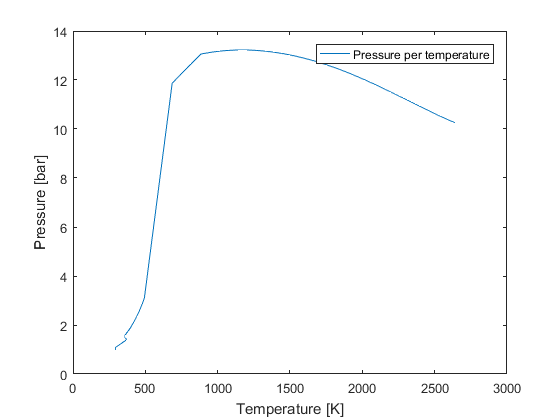
\includegraphics[width=\textwidth]{PperTsimonly}
% 	\caption{Pressure per temperature plotted over the simulated timespan in figure \ref{fig:peakBurn2wsim}. As the temperature rises, the pressure falls.}
% 	\label{fig:pressurepertemp}
% \end{figure}
